%\section{Course structure}
%The course structure: 
%\begin{itemize}
%	\item 10 lectures
%	\item Hopefully a study visit
%	\item Project, mini lecture and corresponding exam questions. Approx 25min. This will give a 20\% bonus in the exam. 
%	\item Written exam 
%\end{itemize}

\section{Course concepts}
The aim of the course is to give a unified perspective on the variety of digital imaging technologies that have been developed the last decades. Different aspects of the imaging technologies will be discussed such as: 
\begin{itemize}
	\item What they are imaging
	\item How 
	\item With what quality
	\item For which applications 
\end{itemize}

After this course you should be able to 

\begin{itemize}
	\item Describe the \textbf{physics} and \textbf{techniques} behind modern imaging techniques
	\item Describe the basic principles for sample preparation in relation to the imaging technique.
	\item Reason and analyze around possibilities and limitations in resolution with regards to:
	\begin{itemize}
		\item density
		\item space
		\item time
		\item spectrum
	\end{itemize}
	\item Describe how the techniques affect the image and subsequent interpretation and analysis
	\item Reason about suitability of different imaging techniques in combination with image processing and machine learning for different applications. 
\end{itemize}

The subject of imaging is interdisciplinary and cover a lot of subjects:

\begin{itemize}
	\item Physics
	\begin{itemize}
		\item Optics, wave propagation
		\item Solid state sensing principles
	\end{itemize}
	\item Electronics
	\begin{itemize}
		\item Circuit designs
		\item Sensor technology
		\item Signal processing
	\end{itemize}
	\item Mathematics
	\begin{itemize}
		\item Geometry
		\item Fourier analysis
	\end{itemize}
	\item Computer science
\end{itemize}

No one is an expert on all imaging technologies and the course therefore consists of lectures of several guest lecturers. They will try to keep it in the common structure. 

\section{What is an image}
An image is a multidimensional sample of the reality that consists of: 

\begin{equation}
D = F(x,y,z,w,t)
\end{equation}

\begin{wbox}{}
\begin{itemize}
	\item Densitometry \textbf{D}, signal intensity
	\item The spatial dimensions \textbf{x,y,z}
	\item Spectral dimension \textbf{w} – wavelength
	\item time \textbf{t} - the temporal dimension 
\end{itemize}
\end{wbox}

We don't have any 5D sensors so we need to \textbf{multiplexing}. Since the subject is digital images, each dimension and the function value must be \textbf{quantized} into a limit range of discrete values. 

The densiometric aspect \textbf{D} or intensity, what physical property is being imaged? is it a reflection, transmission of light, a density distribution of a molecule, a surface topology or an elastic property of an object? How well can we describe this property? and what physical effect do we use to measure: photo resistance, inducted charge or photon counting? 

We create images from signals that can be of different types: electromagnetic waves (light, thermal, x-rays), pressure variations (sound) or contact forces (Braille).

We can use more than only the visible part of the electromagnetic spectrum, we can use all of it with different techniques. 

\subsection{Emission, excited emission, transmission or reflection}
Imaged physical properties can be categories into : \textbf{Emission} (Astronomy, Autoradiography), \textbf{Exited emissions} (Flourescense), \textbf{transmission} (light microscopy, film scanning, classical x-rays) and \textbf{Reflections} (Normal photography, Document scanning, satellite sensors)

Consider where/what is the light source. In case of \textbf{emission} we have a well defined spectral properties, coming directly from the source. \textbf{Transmitted light} on the other hand is exponentially absorbed with a logarithmic intensity that is directly proportional to the absorbing matter. In the case of \textbf{reflection} is the surface orientation as well as the material properties and the direction and the spectral characteristics of the illumination that determines the signal. There is a need to differentiate between diffuse and specular reflection. 

The illumination can be controlled in the case of a \textbf{Active} sensor system. This can be done either all at once for the whole scene or by scanning a pixel or a line at a time. An important example of a \textbf{Active} sensor system is: \textbf{LIDAR:} "laser imaging, detection and ranging".

\subsection{Densitometric aspects: Resolution}
It is important to consider what the densitometric resolution is and what is the signal to noise rate SNR. What pixel depth can we get or in other words how many greylevel do we get and are all of them meaningful. And what is the actual property that is measured? 

\begin{itemize}
	\item Material density
	\item Density
	\item Energy
	\item Photon count
	\item Topographic elevation
\end{itemize}

The contrast resolution is another aspect, the image should have a correct exposure time such that we use the most of the dynamic range of the sensor, not blowing up the brighter parts or under expose the image not showing any details in the darker parts of the image. Using most of the dynamic range of the sensor should result in white noise in the least significant bit. The optimal use of bits is therefore where we have about 1 bit of noise. If the conditions for imaging allows it, it can be possible to increase signal to noise ratio by taking the average of multiple exposure according to:

\begin{equation}
	\sqrt{\text{number of exposures}}	
\end{equation}

We also need to have in mind the spatial consistency and ask: Will all positions in the image give the same density value for the same signal, there could be random or systematic variations where systematic variations can be caused be for example defects or imperfections in the instrument/sensor that can be corrected for by calibration or other methods. One tool for correcting imperfections are: shading correction.

Imperfections is not only present considering spatial consistency where different part of the sensor register differently, we can have non linearity behavior of the registered sensor that must be corrected for with calibration. We need to know if the grey value is linearly or logarithmically  related to the physical property we are interested in. In the field of normal photography is the intensity registered by our sensor linearly related to the reflected light and in transmission imaging is the light absorption logarithmically related to the amount of material the light passes through. If calibration is needed then it will be of importance to investigate of stable it is over time. 

\subsection{The spatial dimension (x,y,z)}
Questions regarding the spatial dimensions to have in mind: How are the spatial dimensions \textbf{x,y,x} mapped into the image? Is the image a slice, a projection a depth map or something else? Are there any distortions that make the image not geometrically correct? What is the spatial resolution. Is it possible to get more than 2 dimensions with the available technology? 

The spatial dimension can be mapped as \textbf{projection} that gives a 2D image of reflections from visible surfaces (in 3D) for the sensor or a transmission through the object. A \textbf{distance} image give explicit information as seen from a single point (2 1/2 D). With a \textbf{slice} we select a slice from a volume. \textbf{Tomographic reconstruction} is a method to compute information about the internal density structure using measurements of numerous line integrals. 

The spatial resolution is limited in different ways in analogue and digital images. In Analogue there are constraints of the aperture of the lens and the wavelength of the light while in digital images the limiting factor is the sampling according to the sampling theorem. Under sampling can give problems such as aliasing and when it is caused be poor sampling the result is often worse then when it is because of limited resolution. It is therefore common to have low pass/blurring filters to prevent sharper images than can be digitized. There have been recent inventions that describes the ways of going beyond the resolution limits. \textcolor{red}{example??} 


Distance images is a wat of representing 3d in 2D by making measurements of the distance to the surface of the object to the sensor for all points in the image. This can be done using either \textbf{passive} sensors with: Parallax camera or stereo images. With an \textbf{active} it can be done with the measurement of time of flight (lidar, radar, ultrasound, laser) or with triangulation, structured light. 

Creating 3D images or image volumes is a rapid growing area in digital imaging mostly driven by medicine. In contrast to the 2D images these can not be viewed directly and it's necessary to use special visualization efforts to interpret the result. These types of imaging system generates very large data sets. Imaging volumes can also be done be psychically slicing (and destroying the sample in the process) and the result would be a 2D image of this thin slice. Another category of volume imaging is \textbf{Tomograpy} that includes: x-ray(CT scan, magnetic resonance (MRI), Emission (SPECT and PET), electron microscopic (EMT) and Optical coherence (OCT \textcolor{red}{what is this?})). Confucal microscopy, ultrasound and holography are also volume imaging techniques.

Reconstructed images like tomographic reconstruction is a type of inverse problem with multiple dimensions that estimates a system from a finite number of projections. Examples of where this technique is used are:

\begin{itemize}
	\item Transmitted X-rays, Computer Tomography (\textbf{CT})
	\item Radioactive decay, Emission Tomography
	\begin{itemize}
		\item PET
		\item SPECT
	\end{itemize}
	\item MRI, emitted excited radio frequency
	\item SAR (synthetic aperture radar)
	\begin{itemize}
		\item CARABAS - long wave - incoherent
	\end{itemize}
\end{itemize}

\subsection{The spectral dimension \textbf{w}}
In all imaging we need to limit the spectral range we are imaging by choosing a range in a wavelength interval. Different spectral ranges often give different image contrast. The signal in each of the pixels is the result of a convolution between:
\begin{itemize}
 	\item The spectral distribution of the illumination
 	\item The spectral absorption/reflection properties of the object.
 	\item The spectral sensitivity function(s) of the sensor. 
 \end{itemize} 

The visual perception by the human eye is the result of the application of the three different spectral sensitivity ranges of the cones. Most imaging system are designed to be optimized for human color reproduction fidelity. There are many different illumination and reflection functions that can give the same color experience. 

For capturing a color image we need three spectral samples which can be captured in different ways where the \textbf{Bayer filter} is the most common. This pattern leads to loss of resolution but is restored by interpolation of some sort. The alternative to having the \textbf{Bayer filter} is to have three sensor chips each color, splitting the image with a prism. This solution is expensive and requires also high mechanical precision. A third option is to stack the three sensing layers for the different color channels which have the benefit of not losing resolution/not need of interpolation. 

\begin{figure}[ht!]
\centering
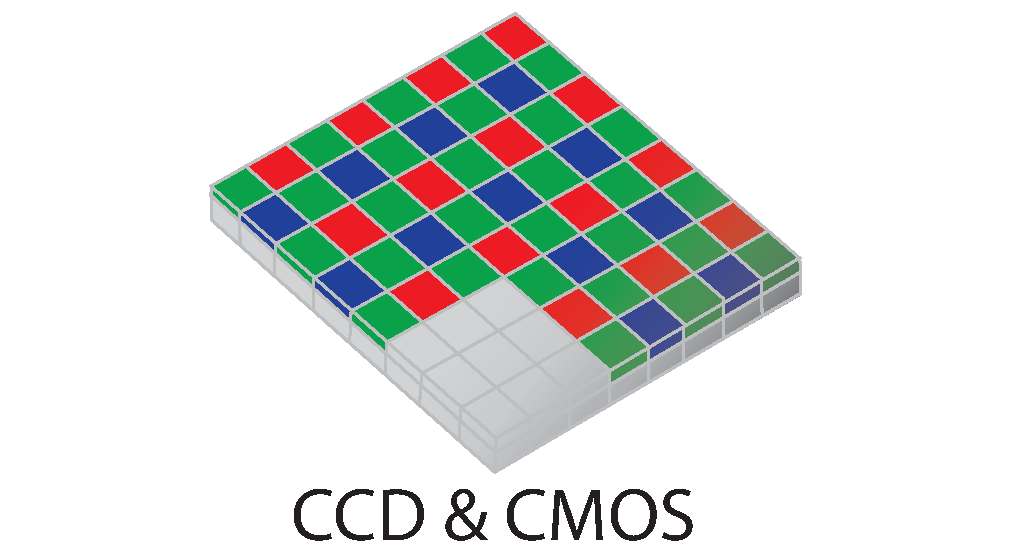
\includegraphics[width=70mm]{figures/CCDandCMOS.pdf}
\caption{Bayer filter}
\label{fig:example}
\end{figure}

What limit us to only use three spectral channels in image analysis is conventional thinking and that there are many cost effective camera in this range. When we register more than one spectral channel we need to use multiplexing, switching between channels either spatially or temporally. Ultimately it should be the application that decides how wide the spectral range should be and the number of channels. It is possible to achieve spectral imaging in a method similar to the Bayer filter, there are cameras with 9 (3 $\times$3) visible light channels and 16 (4 $\times$4) infrared channels that together can give us 25 channels simultaneously. As the number of channels increase to several hundred we call it \textbf{imaging spectroscopy} or hyperspectral imaging. This type of imaging creates a large amount of data and needs effective transmission and compression. 

A solution to capture a large number of spectral channels is to have a rotating filter wheel in front of a wide band, single channel sensor/sensing chip. This requires the scene to be stationary since there will be several images registered.

\subsection{Temporal aspects (\textbf{t})}
Each image will register something for defined time interval and if there is only one single temporal slice we have a still image, while if there are multiple exposures we get a film/movie. For each captured image or exposure we need to define the exposure time, the following questions should be considered:

\begin{itemize}
	\item Does it give motion blur, how fast is the scene/object moving?
	\item Can it be varied freely?
	\item How will the quality of the image be affected by the exposure time? high ISO sensitivity more noise for example. 
\end{itemize}

During the exposure is each pixel, line or image exposed for a certain time, so we need to consider the motion in the scene and of the camera relative to it and the light intensity can by limited. There are however ways to freeze a moving object in the image by using a flash or follow the object in motion with the camera. There are even special solutions with sensors that have electronic object following. 

Using sequences of images can be useful when measuring a motion. It is then crucial with timing:
\begin{itemize}
 	\item Repetition time
 	\item Exposure time
 	\item Data transfer and storage time
 	\item Influenced by resolution in all five dimensions. 
 \end{itemize} 
Sequences can also be used to detect changes in scenes by subtracting the previous stored reference image. For a sequence to be perceived as continuous by the human visual system it is necessary to have a repetition frequency of at least 25 Hz.

Multiplexing is needed since the intensity must be measured for all pixels to get a complete image matrix and we have multiple spectral channels (color RGB) to consider in the integration process. There are no effective sensors that can capture all dimension at once and we need to multiplex the light collection. The amount of parallelism in this light collection is an aspect imaging system and is strongly influenced by how the light is handled (economically) by the system. 

\subsection{Area integration}
Area integration in imaging technology that uses a 2D image sensor to register the light for the whole image in parallel is by far the most common. It started of with image tubes and was later replaced with \textbf{CCD} (Charge Coupled Device) that are now being replaced with \textbf{CMOS} (Complementary Metal Oxide Semiconductor) that could be replaced by new technologies like QIS (photon counting devices) in the future. 

Area integrations gives the best light collection efficiency since it collects "all the light". It also have a rigid geometry and gives stable and predictable imaging geometry that don't suffers from a lot of distortions. There is no need for mechanical motions and they can be mass-produced and therefore inexpensive. The drawbacks with area integration is that it need an even illumination of the whole image surface and there may be varying sensor sensitivities that need to be corrected for. It is also difficult to achieve high fill factor since there are other things that competes for space on the 2D area, multispectral scanning can therefore also be hard to achieve. The image size will be limited by the sensor size. 

CMOS and CCD matrices/sensors are available in many different version with a variety of megapixel resolutions for special applications. In some applications they can be cooled to very low temperatures that allows for long integration times when the light levels are very low. In contrast they can also be used to capture fast events like laser flashes. 

\subsection{Linewise integration}
This kind of sensors are often find in scanners and can be moved to capture an image of the object, or the object can be moved over the sensor. It is also common in remote sensing like satellites that move along the earth surface. 

The technical advantages with line integrations are much better pointwise integration but worse economy compered to area. In motion the orthogonal line will be "frozen" which can be useful in some applications. It allows the use of the other dimension in a 2D sensor for the wavelength, for RGB and hyper spectral scanners \textcolor{red}{? read more}. It possible to create whats called "intelligent sensors" by having a processor for each pixel. 
The disadvantages are similar to area integration, it needs an even illumination along the scan line, it needs corrections of sensor sensitivity along the line of pixels. The 1D fill factor is important but not often a problem \textcolor{red}{meaning?}. There is also a risk for x-y in-homogeneity because of the widely different methods of scanning.  

\subsection{Point-wise integration}
With this methods we register light from one pixel at a time and it requires motion to create the image. Here we most distinguish between what is moving:
\begin{itemize}
	\item The illumination
	\item The sensor
	\item The object
\end{itemize}
The method is mainly used in stationary conditions such as microscopy or scanning film or paper/document. Examples of applications are Drum scanner which produces very high quality scans of document or film. Other applications:

\begin{itemize}
	\item Flying spot scanner
	\item Microscopy
	\begin{itemize}
		\item Fluorescens
		\item Confocal
		\item Multi-photon
		\item Moving stage
	\end{itemize}
\end{itemize}

Some of the advantages are that it gives maximal possibilities for optimization of the measurement of each pixel and that i can have optimized optical path and sensor. No differences between the sensor properties of the different pixel sensors, i.e. only one pixel. It also have the advantage of not having a limit to the image size. The disadvantages are that it uses the incoming light poorly and need some sort of complex mechanical system for scanning which also results in it being very slow compared to the other methods. 

\subsection{Multiplexing for volume imaging}
A few words about multiplexing and volume imaging; It is possible to register single voxels, a line, a plane at a time, the whole volume in parallel. Collecting data in the Fourier domain or through other transforms can be done. Today most tomographic systems collect data from the whole volume or from multiple planes simultaneously which is fast and therefore saves time and signal economy. 

\subsection{Wavefront imaging}
Is new form of imaging that have high information density. The Wavefront sensing measure the amplitude and phase of the incoming optical field simultaneously. It is still under development but show promising results. 

\subsection{Stored intermediate analogue image}
This category is mainly of historic interest and a few example are listed here:

\begin{itemize}
	\item Photographic film
	\item Polaroids
	\item Magnetic tape 
	\item Semiconductor materials (image plates)
\end{itemize}




